\documentclass[11pt,a4paper]{article}
\usepackage[utf8]{inputenc}
\usepackage[spanish,es-tabla]{babel}
\usepackage{amsmath}
\usepackage{amsfonts}
\usepackage{amssymb}
\usepackage{graphicx}
\usepackage{float}
\usepackage{hyperref}
%\usepackage{subfigure} 
\usepackage{amsmath}
\usepackage{amsfonts}
\usepackage[usenames]{color}
\usepackage{subcaption}
\usepackage[left=3cm,right=2cm,top=3cm,bottom=3cm]{geometry}
\author{Gatica, Isaias \\ Martin, Santiago \\ Saez, Lautaro Ándres \\ Vidman, Xavier Harry}
\title{Procesamiento digital de señales: estimación del espectro de una señal aperiódica}
\date{}
\begin{document}
\maketitle
\section{Análisis de una señal aperiódica y discreta}
\label{secc1}
En esta sección se analiza el uso de la DFT para estimar el espectro de una señal aperiódica y discreta. Para ello, se considera en primera instancia la siguiente señal:

\begin{equation}
    x[n]=\delta[n]+\delta[n-1]+\delta[n-2]+\delta[n-3]
    \label{eq.xn}
\end{equation}

Para comenzar el estudio se calcula la DTFT y la DFT de la ecuación (\ref{eq.xn}), a fin de realizar una comparación entre los resultados, y poder concluir si es posible utilizar a la DFT para obtener de forma exacta o aproximada la DTFT de una señal aperiódica.

    \subsection{Relación entre la DTFT y la DFT de la señal x[n]}

	\subsubsection*{Cálculo de la DTFT:}
    Utilizando la definción de la DTFT:
    \begin{equation}
        X(e^{j\omega})=\sum_{n=-\infty}^{\infty}x[n]e^{-j\omega n}
        \label{eq.DTFT}
    \end{equation}
    Donde: 
    \begin{equation}
        \label{omega}
        \omega=2\pi f
    \end{equation}
    Se llega a que la DTFT de la ecuación \ref{eq.xn} es:
    \begin{equation}
        X(e^{j\omega})=1+e^{-j\omega}+e^{-2j\omega}+e^{-3j\omega}
        \label{DTFT.R}
    \end{equation}
    
	\subsubsection*{Cálculo de la DFT:}
    
    Siguiendo con el análisis, se calcula la DFT utilizando la siguiente definición:
    \begin{equation}
        X[k]=\sum_{n=0}^{N-1}x[n]e^{-j\omega_k n} \qquad , 0 \leq k \leq 7
        \label{eq.DFT}
    \end{equation}
    Donde:
    \begin{equation}
        \label{omega.k}
        \omega_k=\frac{2\pi k}{N}
    \end{equation}
    Obteniendo como resultado:
    \begin{equation}
        \label{DFT.R}
        X[k]=1 + e^{-j \frac{\pi}{4} k} + e^{-j \frac{\pi}{2} k} + e^{-j \frac{3 \pi}{4} k}
    \end{equation}
    
    Al cotejar los resultados obtenidos, se observa que las expresiones son muy similares. La diferencia recae en las frecuencias de las exponenciales. La DTFT expresada en la ecuación (\ref{DTFT.R}) tiene como variable una frecuencia $\omega$ que recorre todos los valores de $f$, dando como resultado un espectro continuo. En cambio, la DFT posee una variable $k$ discreta, que recorre solo los valores enteros entre 0 y $N$. Lo mencionado se puede observar en la figura \ref{fig.3a}.
    
    
    \begin{figure}[htb]
    \centering
	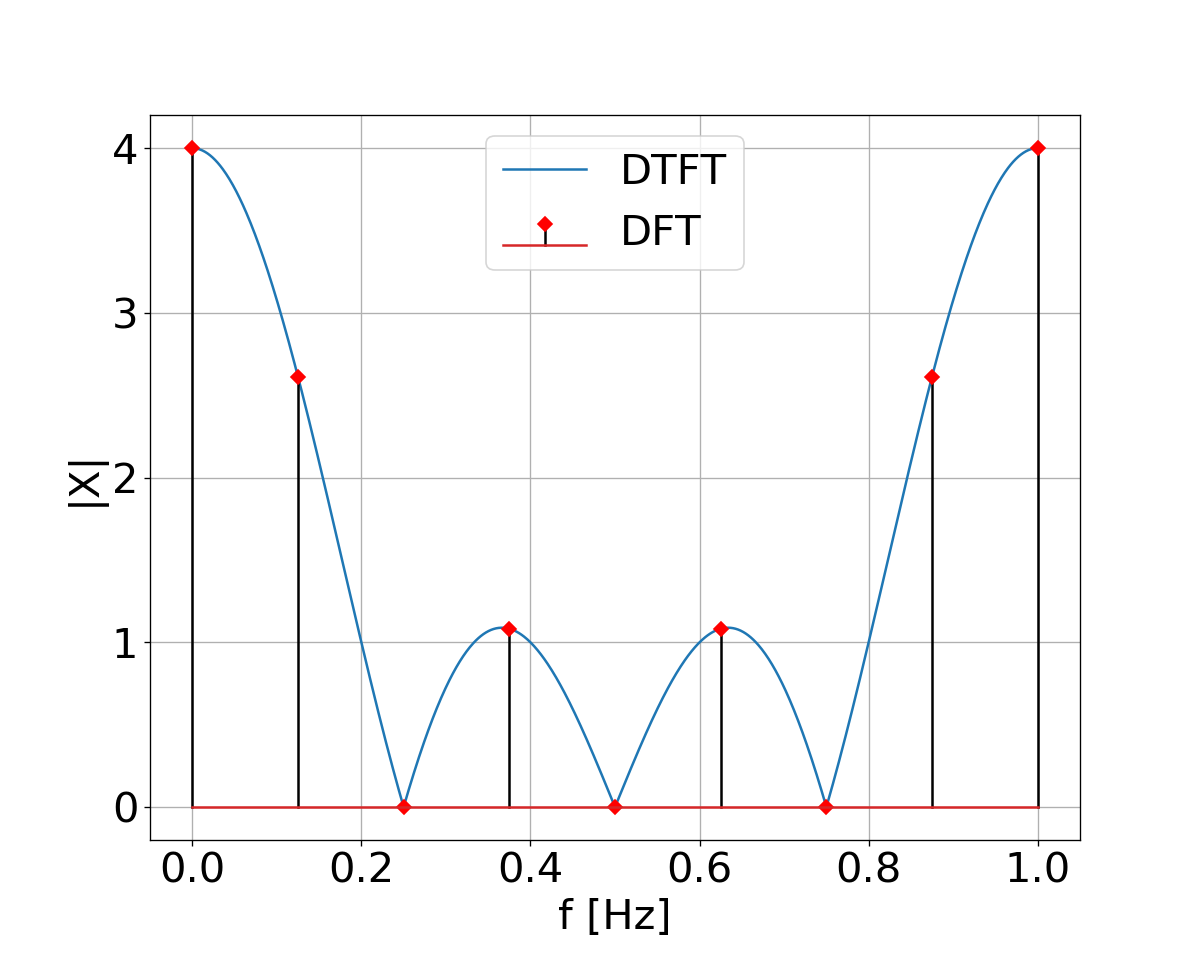
\includegraphics[width=.5\textwidth]{Img/punto_3_a.png}
	\caption{DTFT de la señal $x[n]$}
	\label{fig.3a}
    \end{figure}
    
    Del gráfico mostrado en la figura \ref{fig.3a}, tiene sentido concluir que la DFT muestrea a la DTFT, utilizando los N valores que se le adjudicaron para realizar el cálculo. En la ecuación (\ref{omega.k}) se aprecia como la DFT discretiza la frecuencia angular, dando como resultado que sobre dicha transformada, la DTFT actúe de envolvente. Sin más preámbulos, se afirma que la DFT obtiene de forma exacta a la DTFT en los N valores.
    
    
    %Al comparar los resultados, ecuación \ref{DTFT.R} con ecuación \ref{DFT.R}, se observa que la diferencia recae en la frecuencia. Debido a esto, en la ecuación 
    %\ref{DTFT.R} la frecuencia asociada es la ecuación \ref{omega} que toma valores para todo $f$ dando como resultado un espectro continuo en frecuencia. Esto es un incoveniente a la hora 
    %de realizar el cálculo numérico (por los infinitos valores).Por esto para la \textit{DFT} se discretiza la frecuencia angular dando como resultado la ecuación \ref{omega.k}. Se concluye que es imposible encontrar de forma exacta la \textit{DTFT} a partir de la \textit{DFT}. En otras palabras, se puede decir que 
    %la \textit{DFT} muestrea el espectro continuo de la \textit{DTFT}.

    \subsection{Cálculo de la DFT con distintos puntos}    
    Continuando con el estudio de la DFT, se realiza su cálculo de forma numérica utilizando la \textit{fft}. Para llevar esto a cabo, se genera la señal de la ecuación (\ref{eq.xn}) para los siguientes valores de N: 3, 4 y 8. Los resultados de los tres casos están presentados en la figura \ref{fig.3b}, junto con una señal punteada que corresponde al espectro real de la señal $x[n]$:

    \begin{figure}[htb]
    \centering
    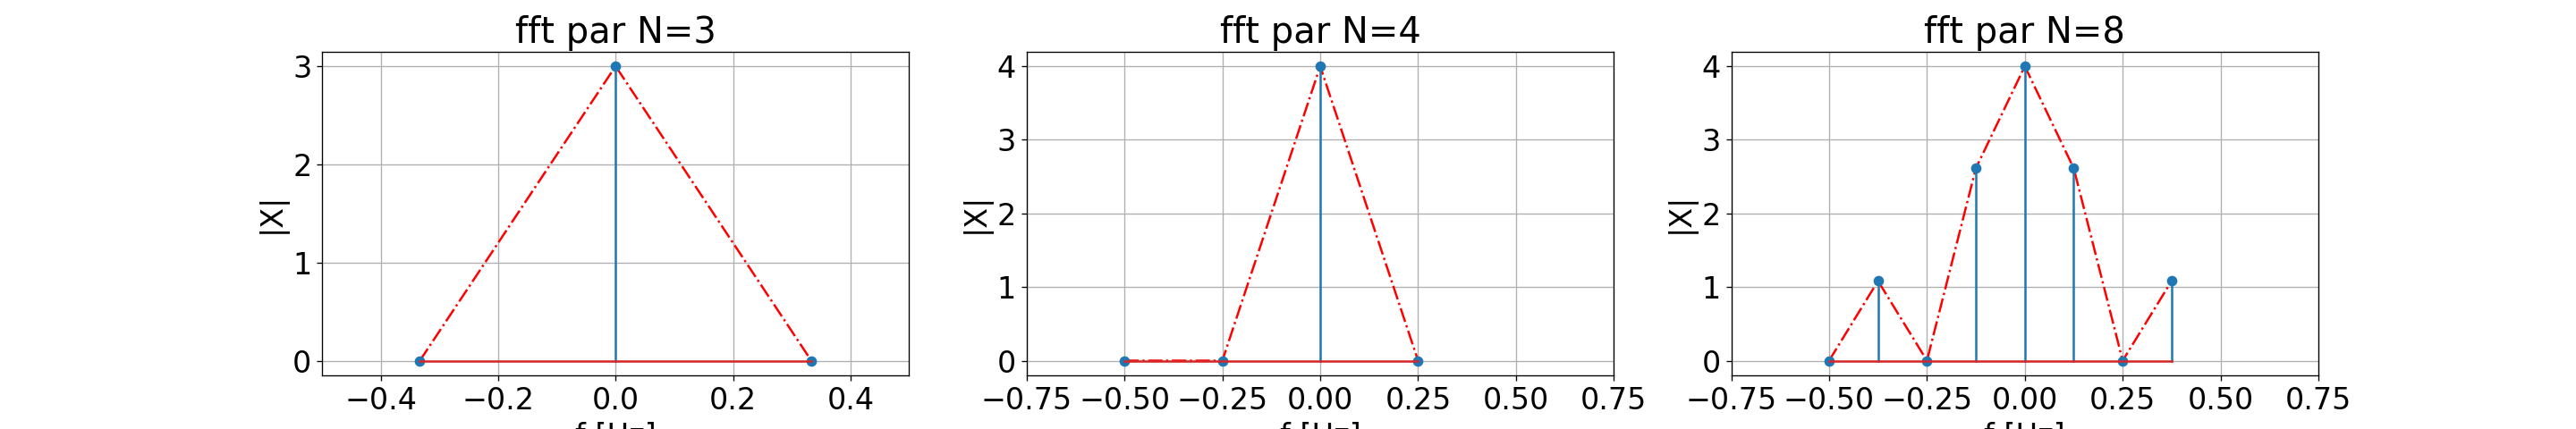
\includegraphics[width=\textwidth]{Img/punto_3_b.png} 
    \caption{Espectros generados con N=3, N=4 y N=8.}
    \label{fig.3b}
    \end{figure}
    
    Analizando los resultados de la figura \ref{fig.3b}, se puede ver que tomar 3 puntos de la señal original difiere con los resultados de la envolvente, y al continuar realizando pruebas con otros valores de N, se observa que al tomar valores de $N$ por debajo de 4, el espectro obtenido a través de la \textit{fft} posee valores diferentes al original. Esto sucede porque se está recortando la señal $x[n]$, y por ende, perdiendo información, lo que termina en un espectro erróneo.
    Asimismo, los valores de la DFT coinciden con el valor de la envolvente en los casos que $N=4$ y $N=8$. Extrapolando estos resultados, se puede decir que para cualquier valor de $N$ mayor a 4, los valores calculados por la \textit{fft} coinciden con los valores de la envolvente.

    \subsection{DFT con zero-padding}
    En esta sección, se realiza el cálculo de la DFT de la señal (\ref{eq.xn}), pero esta vez, con el objetivo de estudiar el efecto del \textit{zero-padding}. Dicho efecto consiste en rellenar con ceros una señal hasta un número determinado de puntos. En este caso, se tomaron las señales anteriores (valores de N: 3, 4 y 8) y se rellenaron con ceros hasta tener 256 puntos, para luego calcular su DFT mediante la \textit{fft}. Los resultados obtenidos se muestran en la figura \ref{fig.1c}.
    
    \begin{figure}[H]
    \centering
    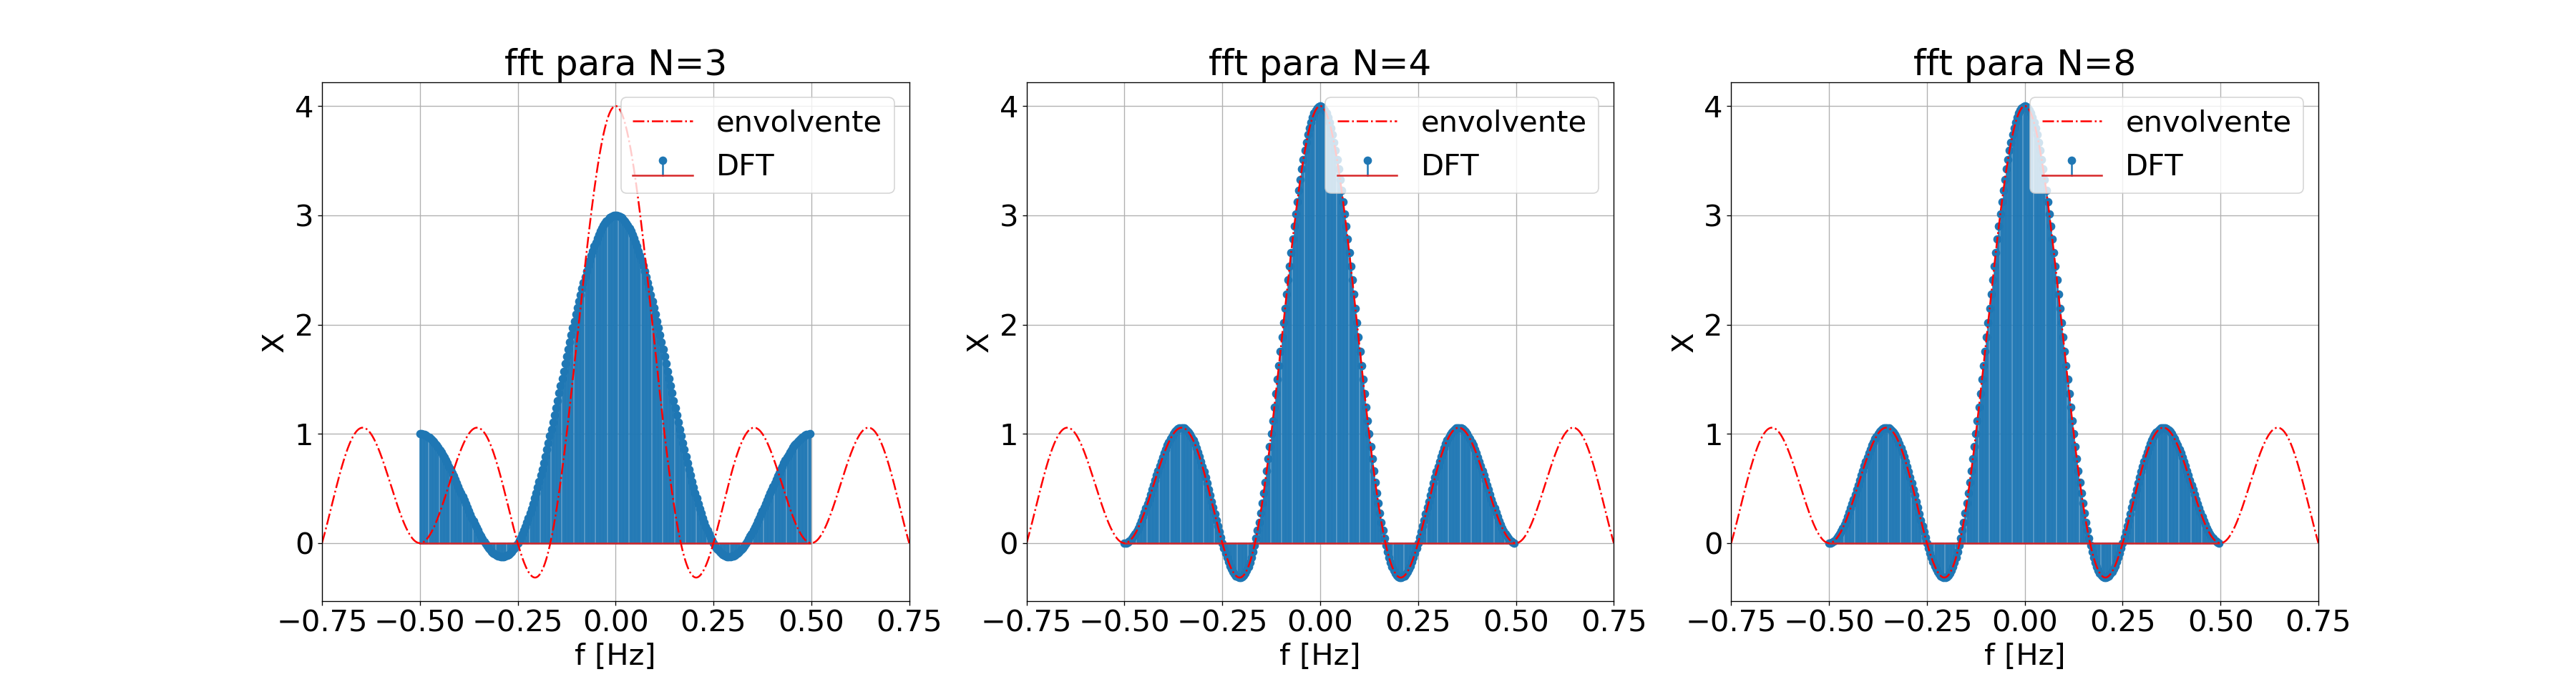
\includegraphics[width=\textwidth]{Img/punto_3_c.png}
    \caption{\textit{fft} con zero-padding hasta 256 puntos para 3,4 y 8 puntos de la señal $x[n]$}
    \label{fig.1c}
    \end{figure}
    
    Al observar la figura \ref{fig.1c}, se concluye que el método \textit{zero-padding} no agrega más información al espectro, sino que solo permite una mejor visualización del espectro real de señal. No obstante, por más que se utilice el \textit{zero-paddding}, si no se realiza con todos los valores distintos de cero de la señal $x[n]$, la aproximación seguirá siendo incorrecta.
    
    %Ahora es posible observar de mejor manera, lo comentado en el apartado anterior, como el zero-padding no agrega mas información al espectro sino que permite una mejor visualización del mismo, cuando se toman 3 puntos de la señal original, no se llega a tomar la señal completa si no que se recorta, por lo que el espectro si bien un aspecto similar, es mas ancho y de menor amplitud (al ser un cajon de 3 puntos y no de 4 puntos como la señal original), y para los casos de N=4 y N=8 que si se utiliza toda la información de la señal $x[n]$ se ve claramente que los valores de la DFT corresponden a muestras de la DTFT.


    \subsection{Cálculo de la DTFT utilizando la \textit{fft}}
        En el siguiente apartado se concluye sobre las condiciones necesarias que debe tener una señal aperiódica, para lograr aproximar de una manera correcta el cálculo de su DTFT con el algoritmo \textit{fft}. 
        
        
        De los análisis anteriores se sabe que la DFT muestrea al espectro continuo de una señal $x[n]$ aperiódica. La siguiente ecuación expresa la relación que hay entre la frecuencia discretizada de la DFT con la frecuencia de la DTFT: 
        
        \begin{equation}
            X[k]=X_{DTFT}\left(  \frac{2 \pi}{N} k \right)
        \end{equation}

        Donde $N$ es el número de puntos que se utilizan para calcular la DFT.

        No obstante, hay ciertas condiciones que se deben cumplir para lograr un obtención exacta de la DTFT, y por lo tanto, que los valores obtenidos de la \textit{fft} sean considerados muestras del espectro real de la señal. Las condiciones son las siguientes:

        \begin{enumerate}
            \item La señal debe ser de duración finita ($L$).
            \item Al realizar el cálculo numérico, utilizar al menos $L$ puntos.
        \end{enumerate}
    
    \subsection{Código para la obtención de la DTFT:}
    En esta sección se utiliza el código adjunto a este informe para calcular la DTFT de tres señales aperiódicas discretas. En principio, se calcula la DTFT de forma teórica. Luego, se muestra en gráficos el resultado obtenido de forma numérica. Las señales utilizadas son las siguientes:
    \begin{itemize}
    \item \begin{equation}
    x_{1}[n] = \left\{ 
        \begin{array}{ll} 
        n & \mathrm{si\ } 0\leq n \leq 4 \\
        10-n & \mathrm{si\ } 5\leq n \leq 10 \\
        0 & \mathrm{sino\ } \\
        \end{array} 
        \right.
    \end{equation}
    
    \item \begin{equation} 
        x_{2}[n] = \left\{ 
        \begin{array}{ll} 
        1 & \mathrm{si\ } -2\leq n \leq +2, \\
        0 & \mathrm{sino\ } \\
        \end{array} 
        \right.
    \end{equation}
    
    \item \begin{equation} 
        x_{3}[n]=(-0,5)^{n}u[n]
    \end{equation}

    \end{itemize}   
    
    A continuación, se pueden observar los resultados de la DTFT de forma numérica en las siguientes figuras:
    
    \begin{figure}[H]
    \centering
    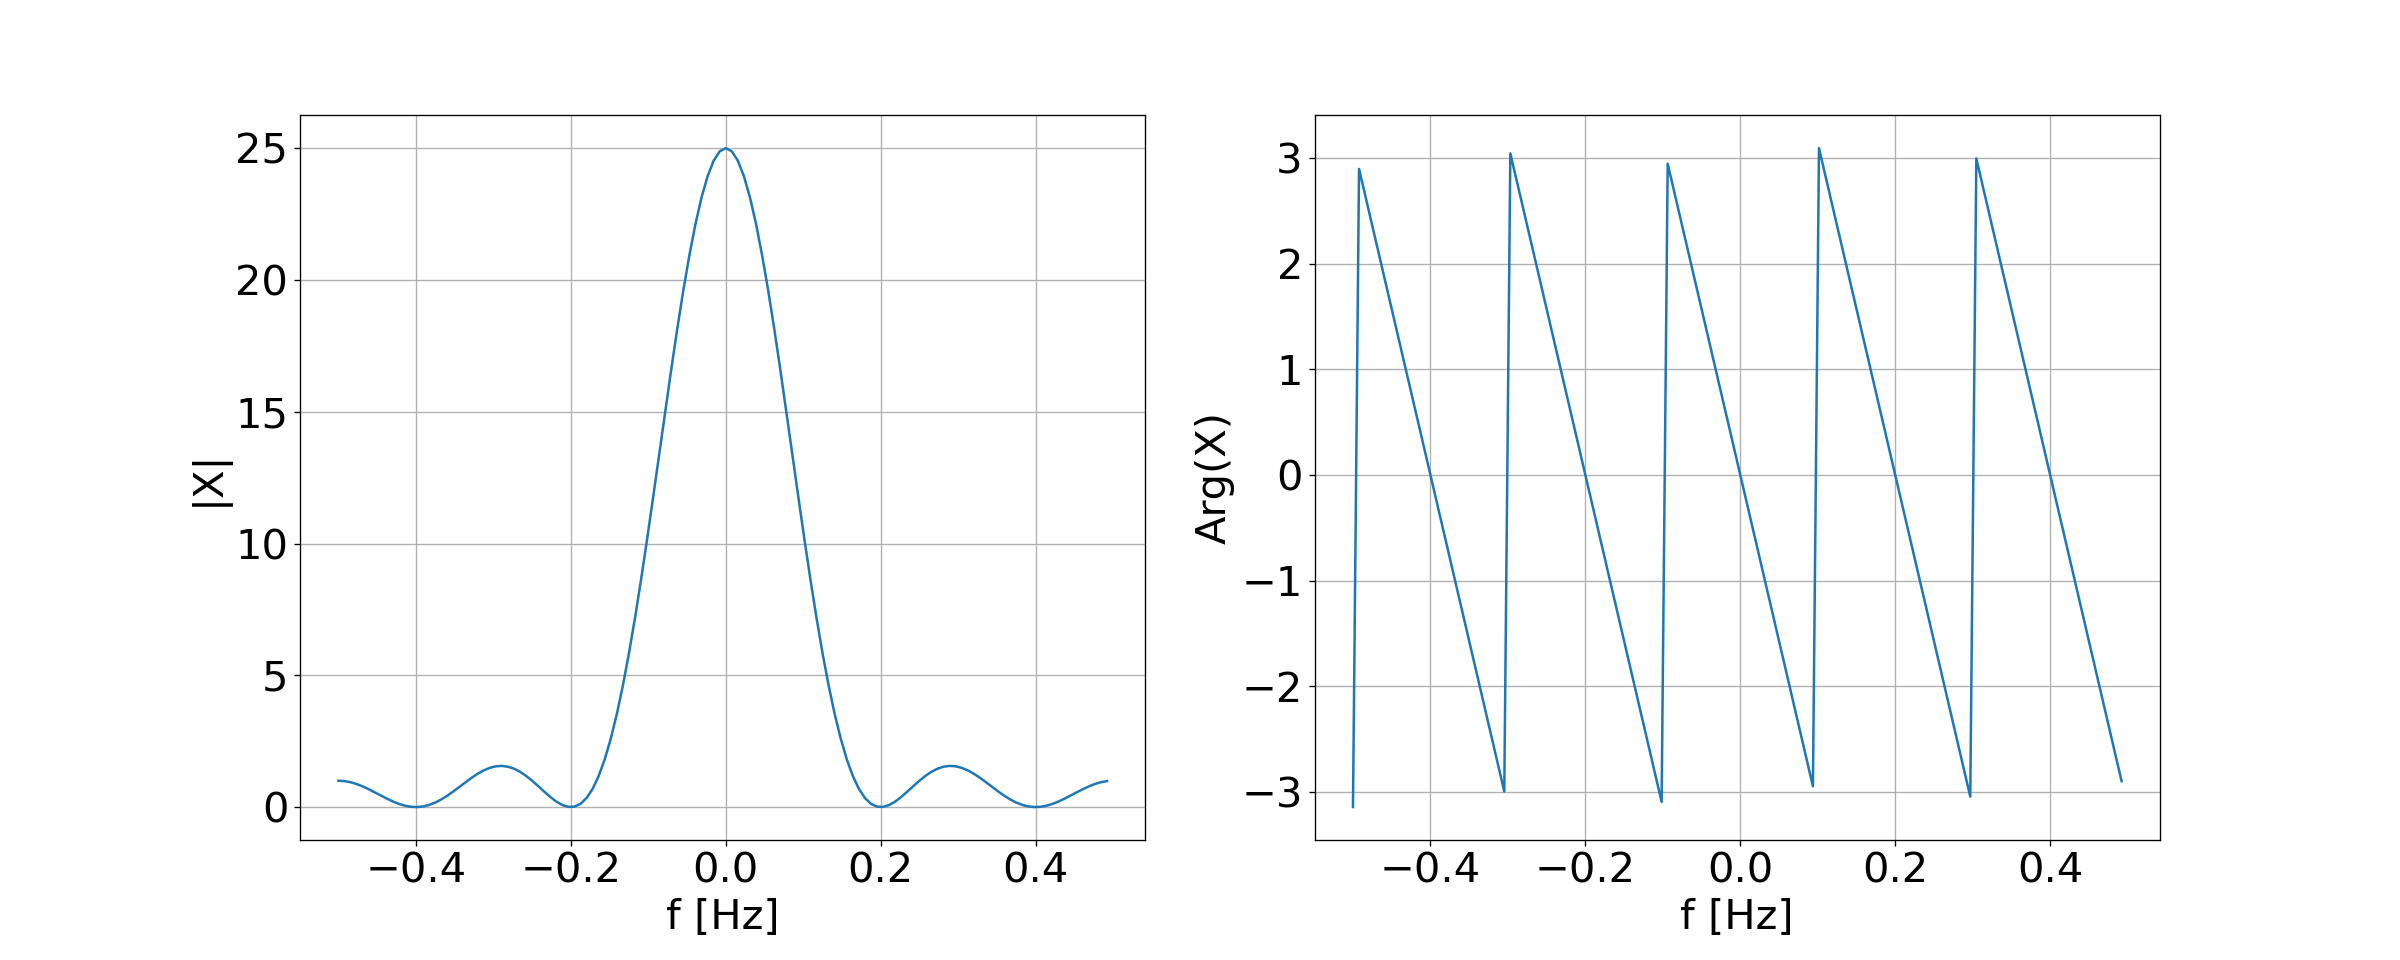
\includegraphics[width=\textwidth]{Img/punto_3_e_1.png}
    \caption{espectro de la señal $x_{1}[n]$ mediante el algoritmo.}
    \label{fig.3ei}
    \end{figure} 


    \begin{figure}[H]
    \centering
    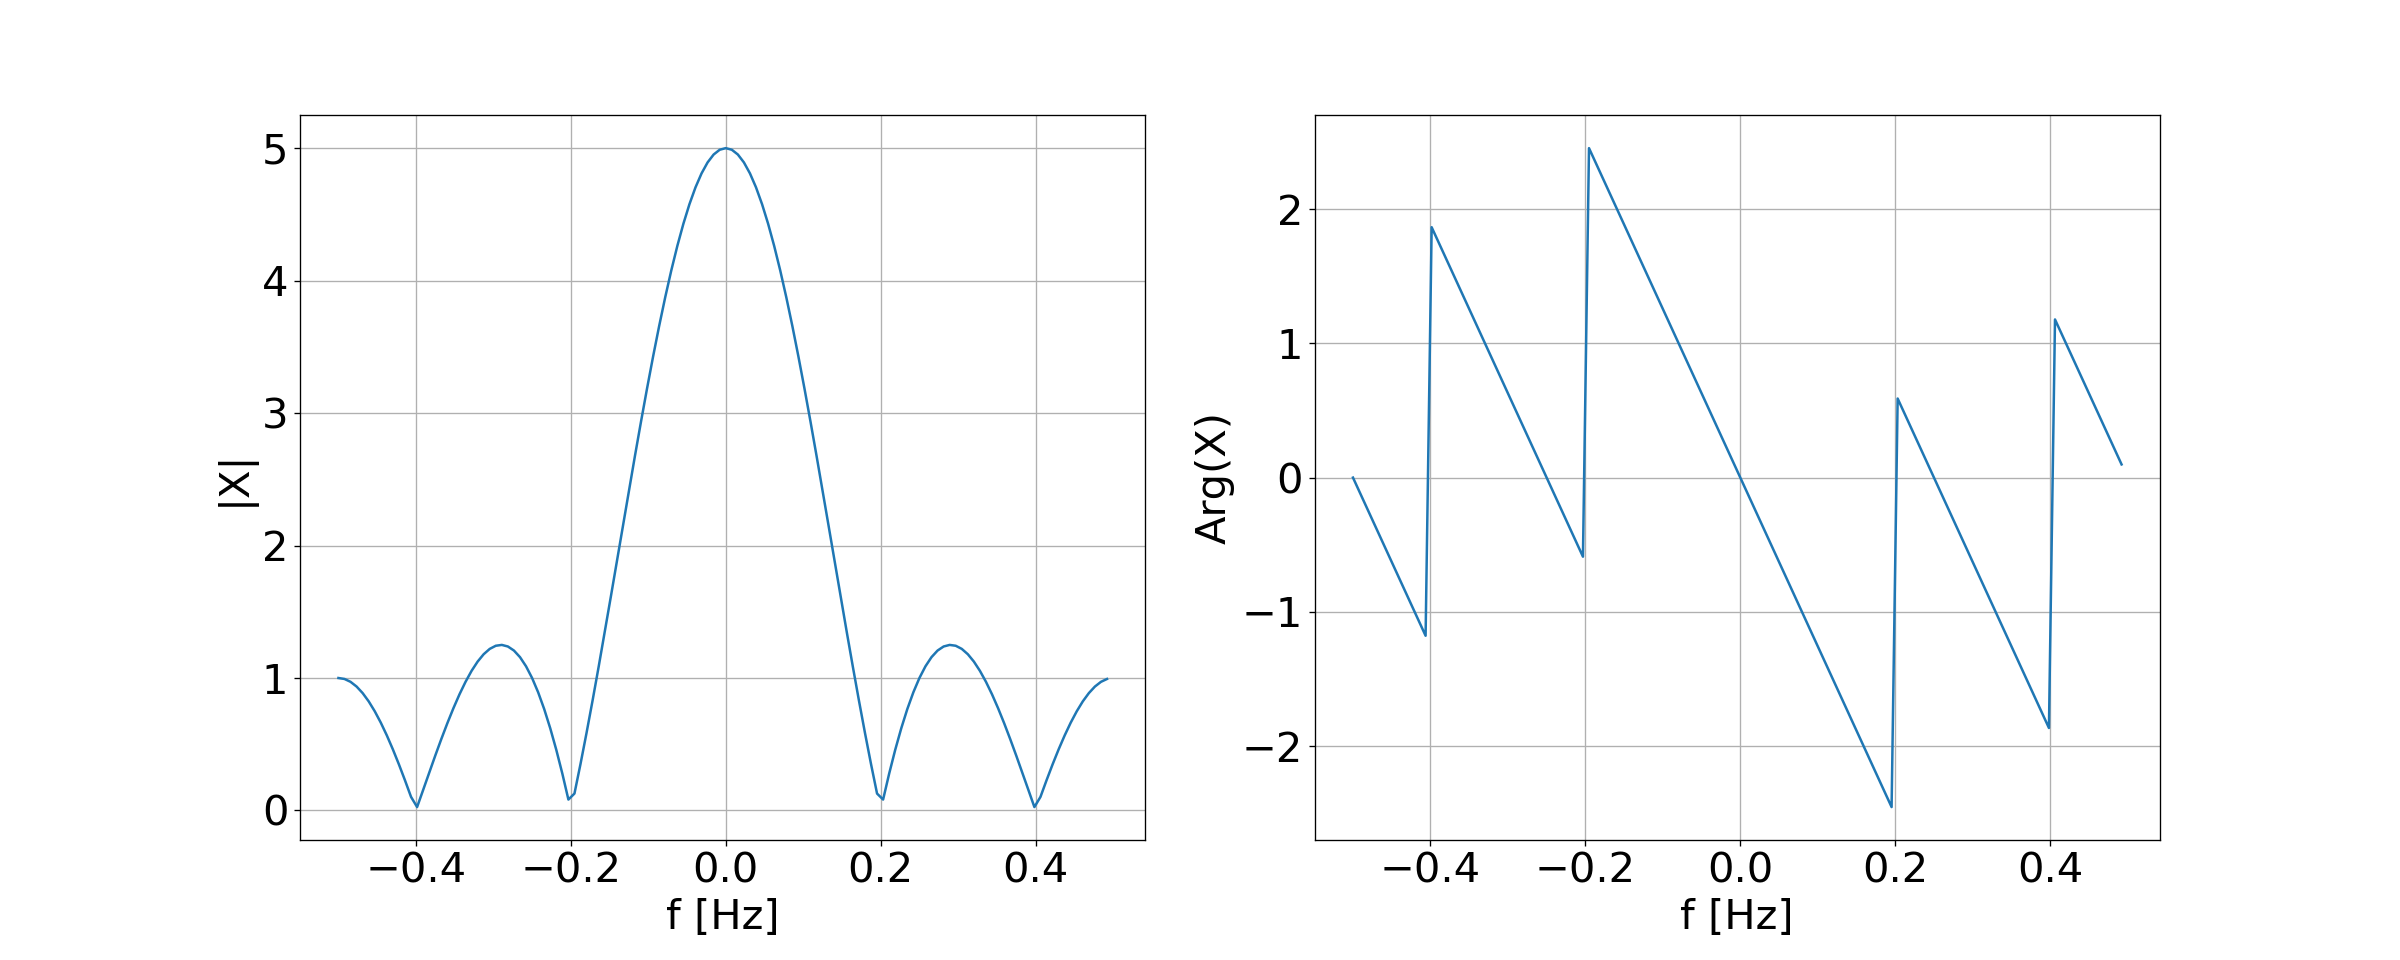
\includegraphics[width=\textwidth]{Img/punto_3_e_2.png}
    \caption{espectro de la señal $x_{2}[n]$ mediante el algoritmo.}
    \label{fig.3eii}
    \end{figure}


    \begin{figure}[H]
    \centering
    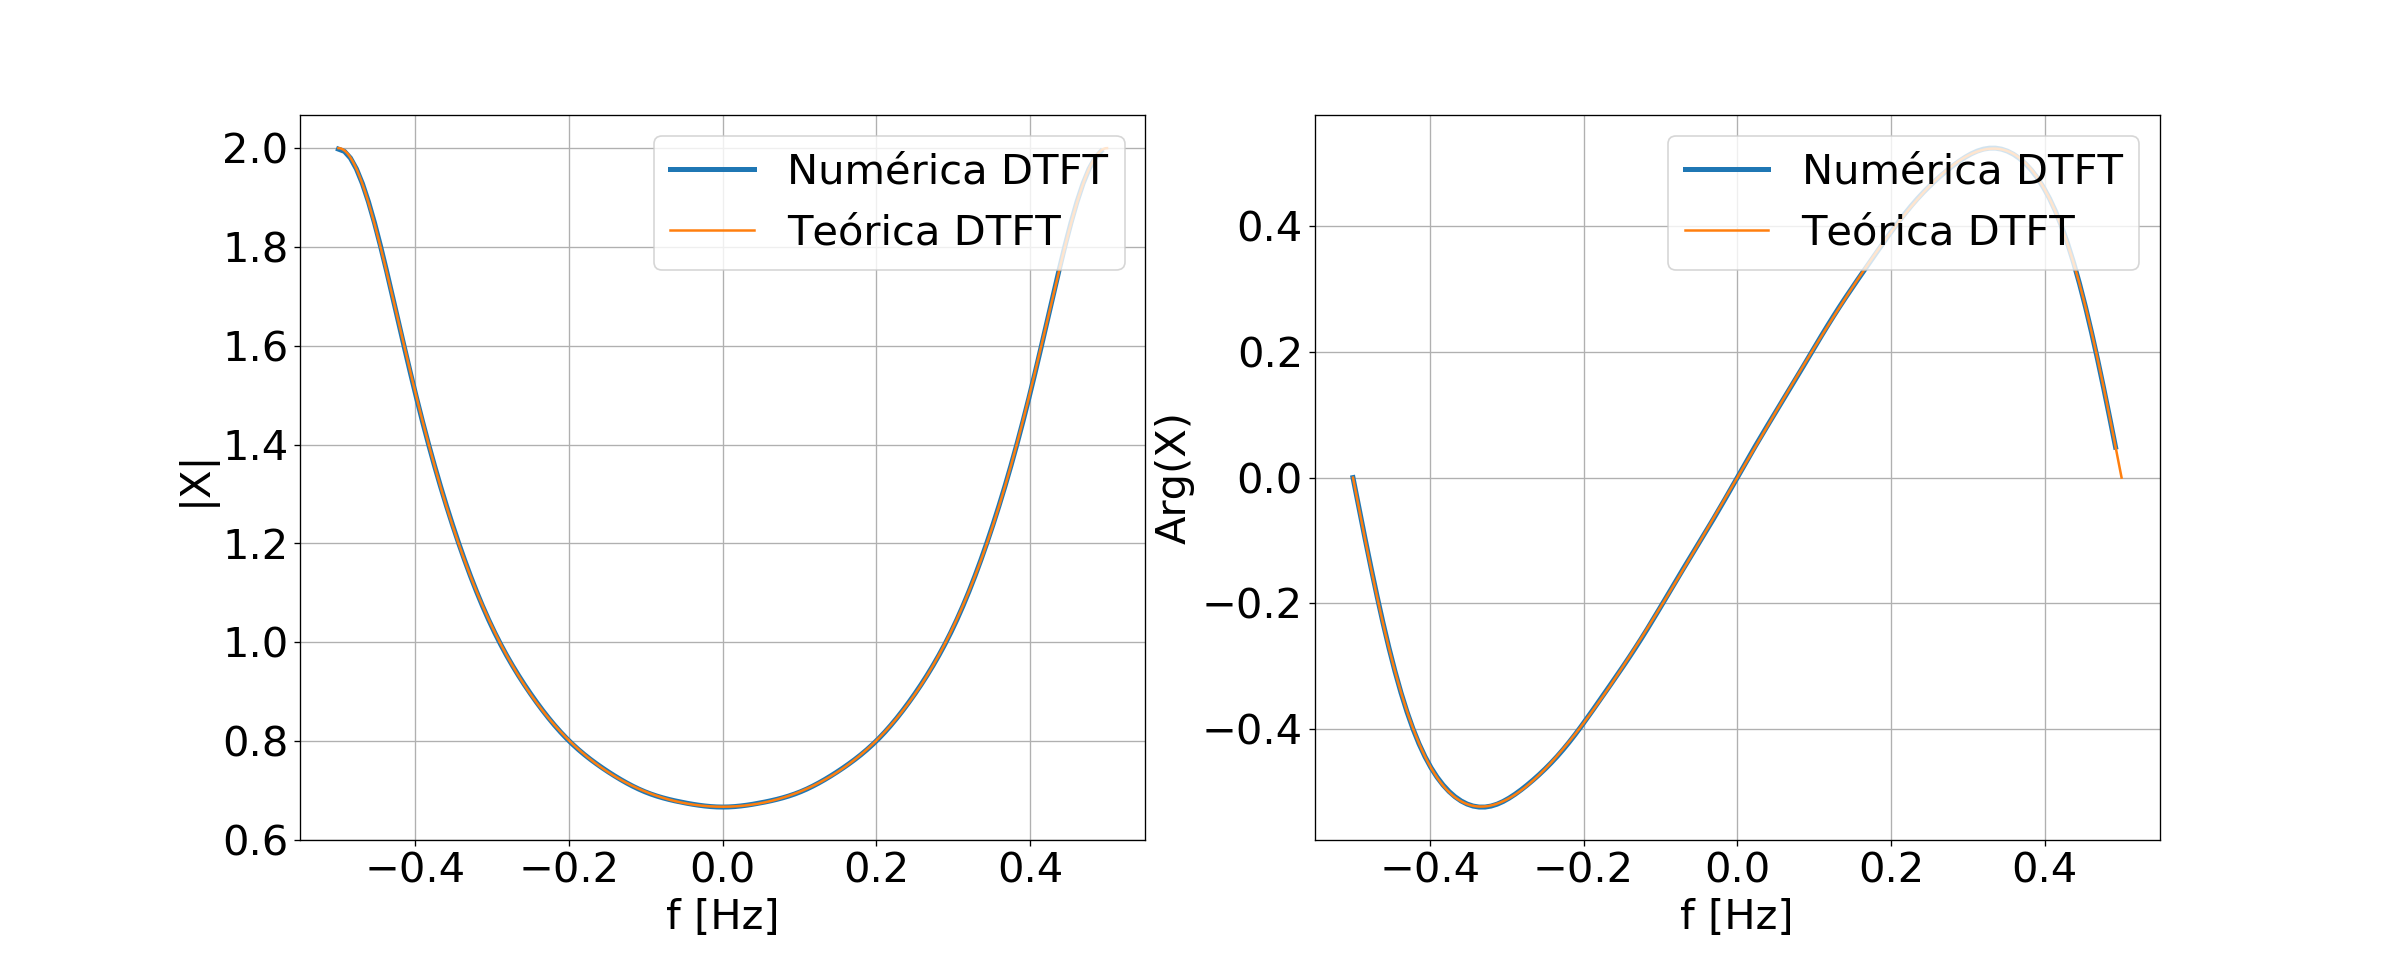
\includegraphics[width=\textwidth]{Img/punto_3_e_3.png}
    \caption{espectro de la señal $x_{3}[n]$ mediante el algoritmo.}
    \label{fig.3eiii}
    \end{figure}

    Se puede apreciar que los espectros representados en las figuras \ref{fig.3ei},\ref{fig.3eii} y \ref{fig.3eiii} coinciden de manera aproximada con lo obtenido de manera teórica. 
    
    
%\begin{figure}[htb]
%\begin{subfigure}{.6\textwidth}
%  \centering
  % include first image
%  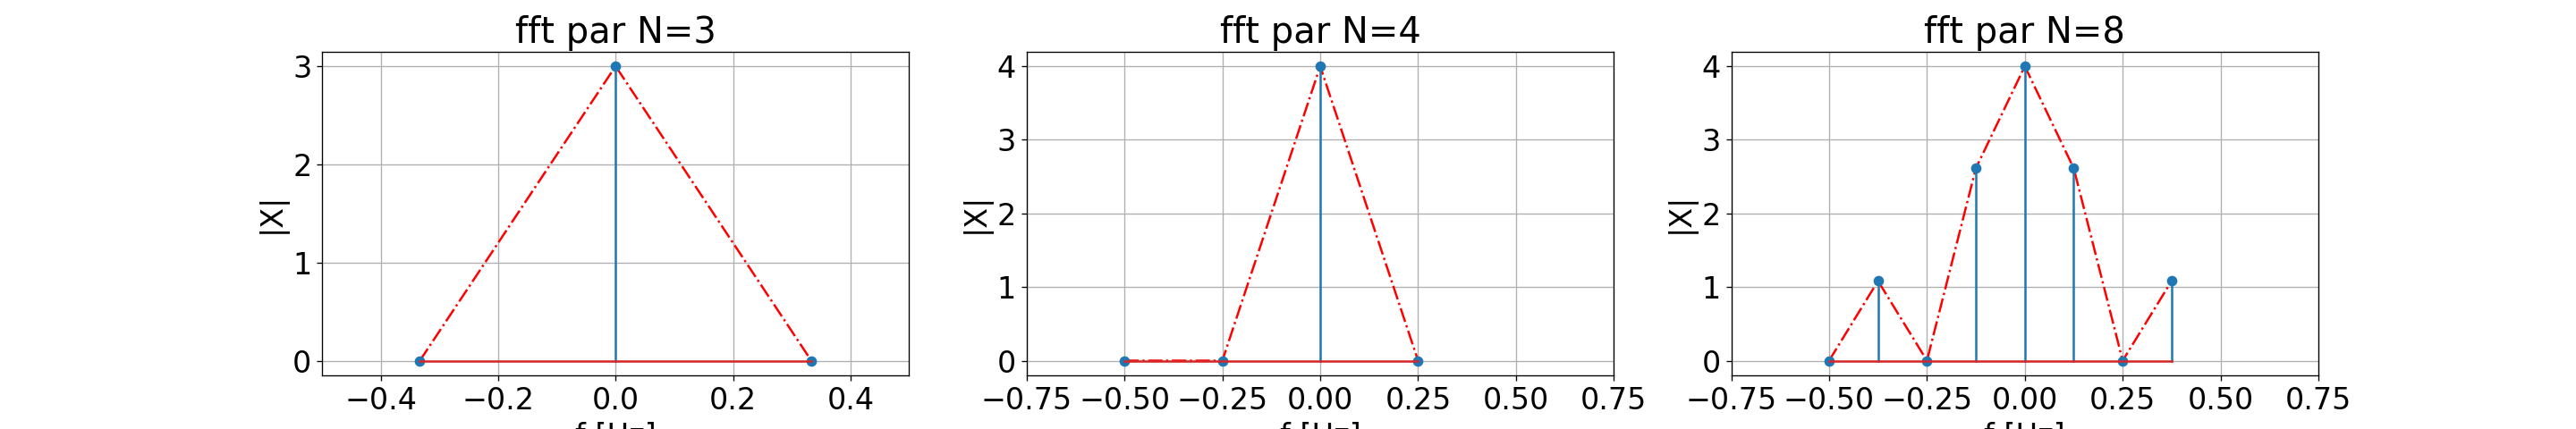
\includegraphics[width=.8\linewidth]{Img/punto_3_b.png}  
%  \caption{Put your sub-caption here}
%  \label{fig:sub-first}
%\end{subfigure}
%\begin{subfigure}{.6\textwidth}
%  \centering
  % include second image
%  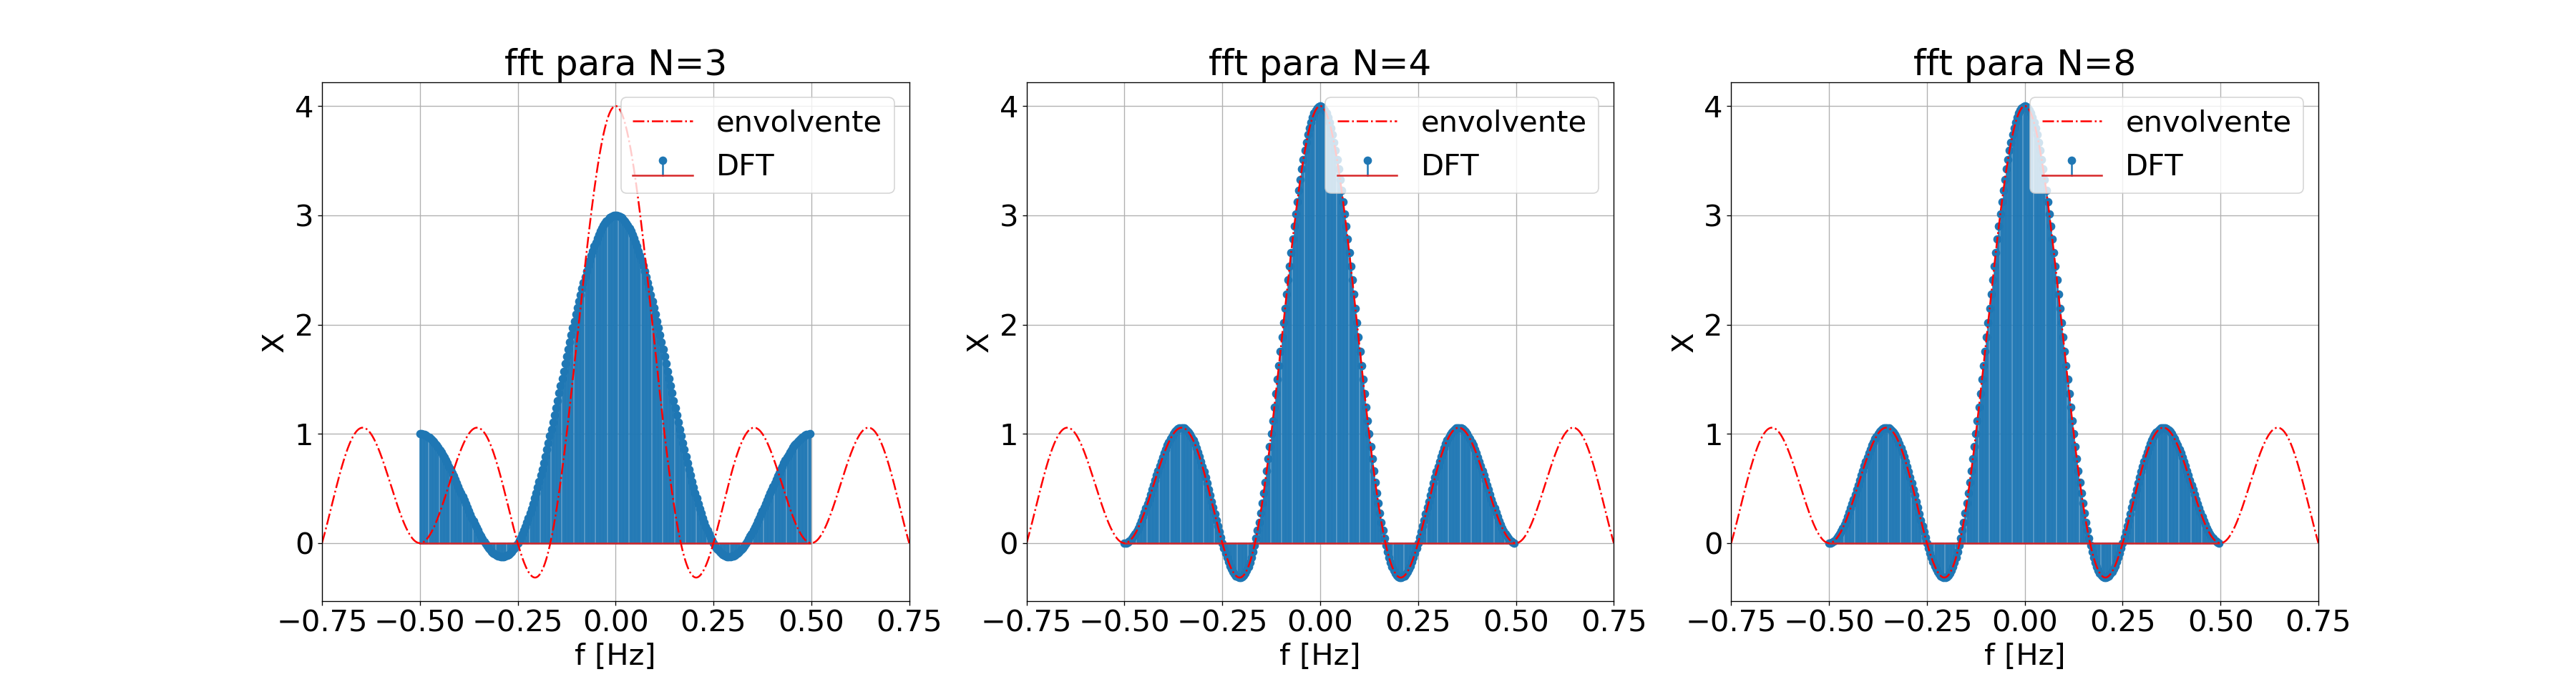
\includegraphics[width=\linewidth]{Img/punto_3_c.png}  
%  \caption{Put your sub-caption here}
%  \label{fig:sub-second}
%\end{subfigure}
%\caption{Put your caption here}
%\label{fig:fig}
%\end{figure}


\section{Análisis de una señal aperiódica y continua}

En el siguiente apartado se analiza el uso de la DFT para estimar el espectro de una señal aperiódica y continua. Para comenzar el estudio, se considera la siguiente señal:

\begin{equation}
    x(t)=u(t-3)-u(t)
    \label{eq.xt}
\end{equation}

A continuación, se calcula la CTFT de la señal $x(t)$ y, realizando un muestreo apropiado (cumpliendo con el teorema de muestreo) de $x(t)$, se calcula la DFT de la señal $x[n]$ obtenida a partir de $x(t)$. El cálculo de la CTFT y la DFT son con el objetivo de hallar relaciones entre dichas transformadas.

\subsection{Relación entre la CTFT, DTFT y DFT de la señal $x(t)$}

\subsubsection*{Cálculo de la CTFT:}

Utilizando la definción de la CTFT:

\begin{equation}
    X(j\Omega)=\int_{-\infty}^{\infty} x(t)e^{-j\Omega t}dt
\end{equation}

Luego, analizando que la señal $x(t)$ resulta ser un cajón de amplitud negativa en el intervalo del tiempo $0\leq t \leq 3$, se puede calcular la CTFT de la siguiente forma:

\begin{equation}
    X(j\Omega)=\int_{0}^{3} -1e^{-j\Omega t}dt
\end{equation}	

\begin{equation}
    X(j\Omega)=\frac{1}{j\Omega} \left[e^{-j\Omega t} \vert_{3}^{0}\right] = \frac{e^{-3j\Omega} - 1}{j\Omega}
\end{equation}

Trabajando la expresión anterior se llega al siguiente resultado:
\begin{equation}
    X(j\Omega) = -3e^{\frac{-3j\Omega}{2}} sinc(3F)
\end{equation}

\subsubsection*{Cálculo de la DFT:}

Por otra parte, para el cálculo de la DFT se muestrea la señal $x(t)$ utilizando una frecuencia de muestreo $F_s=1Hz$, con la intención de obtener cuatro muestras de la señal original. El resultado de este muestreo es igual a la ecuación (\ref{S.disc}) pero invertida en amplitud. Paulatinamente, se aplica la ecuación (\ref{eq.DFT}) utilizando $N=4$ con el fin de utilizar todas las muestras distintas de cero.

\begin{equation}
    X[k]=\sum_{n=0}^{3}-1e^{-j\omega_k n} = \frac{1 - e^{-j4\omega_k}}{1-e^{-j\omega_k}} = e^{-j\frac{3}{4}\pi k} \frac{sin(\pi k)}{sin(\pi k/4)}
    \label{S.disc}
\end{equation} 

Si se realiza un análisis de las ecuaciones utilizadas para el cálculo de la DFT y la DTFT, siendo la ecuación de la DTFT:
 
\begin{equation}
    \label{DTFT}
	\tilde{X}(e^{j \omega T}) = \sum_{n=- \infty}^{\infty} x_{c}(nT) e^{-j \omega nT}=\frac{1}{T}\sum_{m=- \infty}^{\infty} X_{c} \left(j \omega - j \frac{2 \pi}{T}	m \right)	
\end{equation}

Donde $x_{c}(nT)$ son las muestras de $x_{c}(t)$.
 
 De la sección \ref{secc1}, se sabe que la DFT muestrea a la DTFT, utilizando los N valores que se le adjudicaron para realizar el cálculo. En la ecuación (\ref{omega.k}) se aprecia como la DFT discretiza la frecuencia angular. Reemplazando dicha relación en la ecuación (\ref{DTFT}) se obtiene la expresión de la DFT:
 
 \begin{equation}
 X[k] = \frac{1}{T}\sum_{m=- \infty}^{\infty} X_{c} \left(j \frac{2 \pi k }{N} - j \frac{2 \pi}{T}	m \right)    , k =0,1..., N-1 \\
 \label{eq.19}
 \end{equation}
 
 quedando entonces expuesta la relación entre ambas.
 
 Por otro lado, analizando la relación entre la DTFT y la CTFT, solo basta con realizar un nuevo análisis de la ecuación (\ref{DTFT}). En ella, se puede ver implícita la relación entre ambas transformadas.
 Por inspección, se visualiza en (\ref{DTFT}) que la DTFT de la señal muestreada no es más que la periodización del espectro de la señal continua original.
 Sin más preámbulos, la relación entre la DTFT y la CTFT es que la DTFT es un espectro periódico con posible aliasing de la señal CTFT.

%EL C
\subsection{Obtención de la CTFT a partir de la DFT para cualquier señal aperiódica continua}  
\label{secc4c}
Para estimar la CTFT a partir de la DFT se puede optar por 2 caminos igualmente validos, estos son :  

\begin{enumerate}  
\item Muestrar la señal $x_{c}(t)$ y se obtiene la señal $x[n]=x_{c}(nT)$, y se calcula la DFT a dicha señal.  
\item Utilizar la ecuacion (\ref{eq.19}).  
\end{enumerate} 

Se puede obtener una estimación exacta si se eligen de manera correcta los siguientes parámetros:  

\begin{enumerate}      
\item Frecuencia de muestreo: se debe elegir una $F_s$ que cumpla el teorema de muestreo. Esta condición se ve reflejada en el \textit{aliasing} resultante del espectro. Si bien el espectro siempre va presentar aliasing (debido a que se esta muestreando una señal aperiódica) éste se puede disminuir al utilizar $F_s$ cada vez mayores.      
\item Cantidad de muestras: se debe elegir una cantidad de muestras $N$ mínima que contenga la información de la señal muestreada. A partir de esta idea se desprenden dos situaciones:      

\begin{itemize}          
\item Señal $x[n]$ de duración finita: En este caso si la longitud de la señal es igual a $L$, la cantidad de muestras debe ser $N \geq L$.          
\item Señal $x[n]$ de duración infinita: En este caso la cantidad de muestras $N$ debe ser lo mas representativa posible, es decir mientras mayor sea $N$ mejor sera la aproximación.     
\end{itemize} 
\end{enumerate}


%EL D
\subsection{Cálculo de la CTFT de la señal x[n] a partir de la \textit{fft}}

Se establece como frecuencia de muestreo $F_s=1Hz$, ya que dicha frecuencia es mayor a 2 veces la frecuencia del primer cero, por lo tanto la señal
muestreada conserva el $90\%$ de la energía de la señal original. Obteniendo:

\begin{equation}
    x[n]=-\mu[n]\mu[3-n]
\end{equation}

En general se puede establecer que para cualquier frecuencia de muestreo $Fs$ se obtiene 

\begin{equation}
    x{F_s}[n]=-\mu[n]\mu[3F_s-n]
\end{equation}

Donde el ancho del pulso esta determinado directamente por el valor de $F_s$.

Luego al realizar una variación de frecuencia se obtiene que a mayor $F_s$ mejor es la aproximación, esto se debe a que el espectro de la 
señal de $x(t)$ no es de banda limitada, y por lo tanto siempre existirá aliasing.

\begin{figure}[H]
    \centering
    %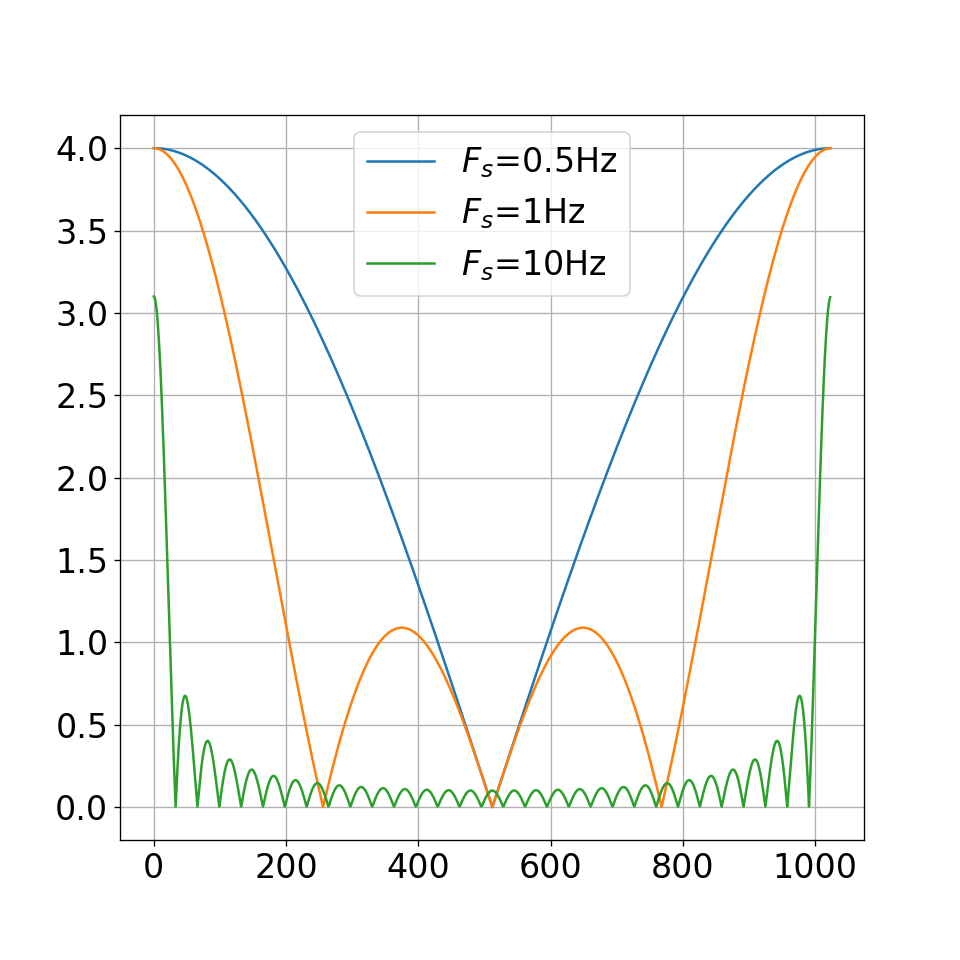
\includegraphics[width=\textwidth]{Img/punto_4_d.png}
    \caption{Aproximacion de la CTFT mediante la \textit{fft} para distintos valores de $F_s$ y con zero padding hasta $1024muestras$.}
    \label{fig.4d}
\end{figure}

Al observar la figura \ref{fig.4d} se observa que para $F_s=1Hz$ es posible recuperar los 2 primeros lóbulos del espectro, pero su amplitud 
tiene un error notorio. Mientras que si se baja la frecuencia a $F_s=0.5Hz$ solo se recupera un solo lóbulo, y el aliasing debido al mal muestreo de la señal es muy notorio. Si se utilizan frecuencias menores a $0.4Hz$ se obtiene una señal continua debido al gran aliasing sufrido por la superposición del lóbulo central. Al aumentar $F_s$ hasta $10Hz$ se observa que la aproximación del espectro mejora mucho en cuanto a la amplitud y se pueden recuperar 
muchos mas lóbulos.

%EL E
 \subsection{Cálculo de la CTFT de x(t) utlizando la \textit{fft} con N=10 y N=1000}
 En la siguiente subsección, se muestrea la señal $x_{c}(t)$ a la frecuencia $Fs=3 Hz$ para obtener una señal $x[n]$, la cual consta de 9 puntos. Luego, se calcula la DFT con 2 valores de N distintos: N=10 y N=1000, obteniendo el siguiente resultado:
 
 \begin{figure}
 \centering
     %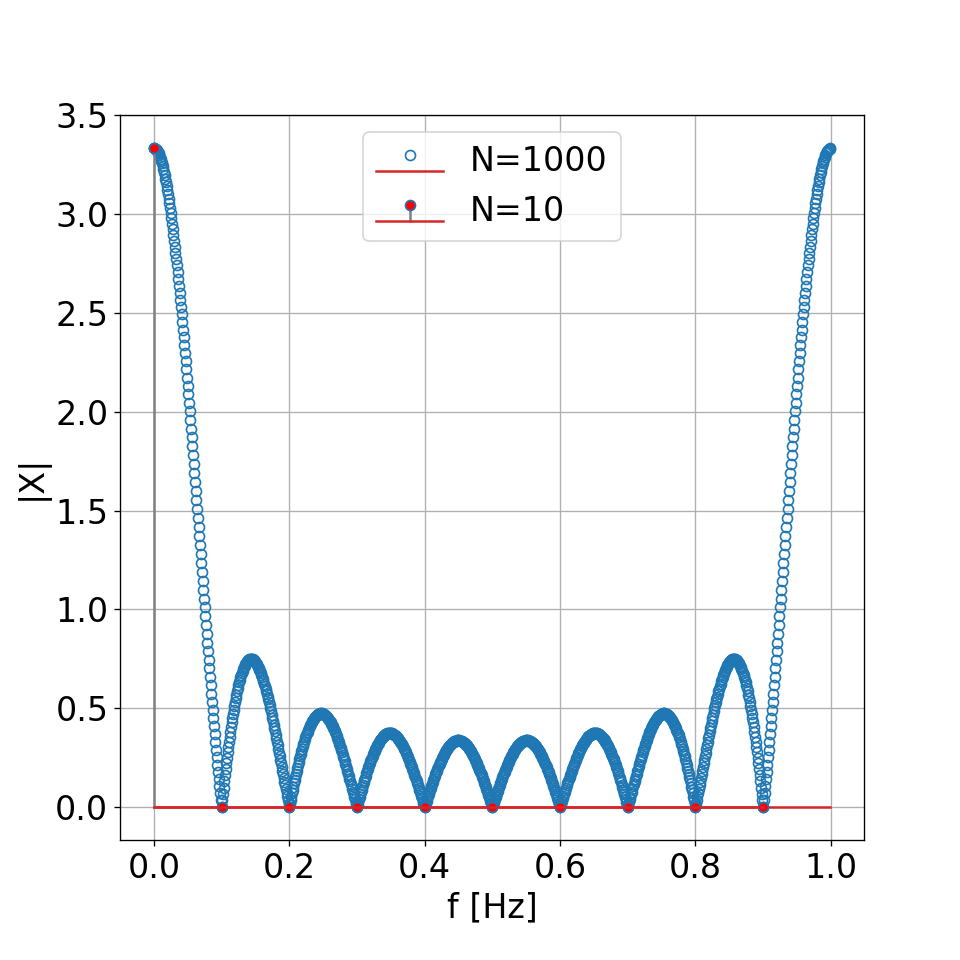
\includegraphics[width=\textwidth]{Img/punto_4_e.png}
     \caption{DFT de la señal x[n] para N=10 y N=1000}
     \label{fig.4e}
 \end{figure}
 Si se observa la figura \ref{fig.4e}, se ve que al utilizar un número mayor de puntos para el cálculo de la DFT, el resultado parecería ser más exacto. Pero como la señal solo contiene 9 puntos distintos de cero, al tomar N=1000 las muestras adicionales no contienen información, y la frecuencia a la que se distribuyen los valores de la DFT en el espectro disminuye (ver la relación en la ecuación \ref{omega.k}). En consecuencia, esto genera una mejor visualización del espectro, pero no agrega información adicional, por lo tanto la estimación de la CTFT es la misma.



%El F
\subsection{Implementación de la función \textit{fftshift}}
Los resultados que se obtienen al utilizar la \textit{fftshift} son:
\begin{figure}[]
    \centering
    %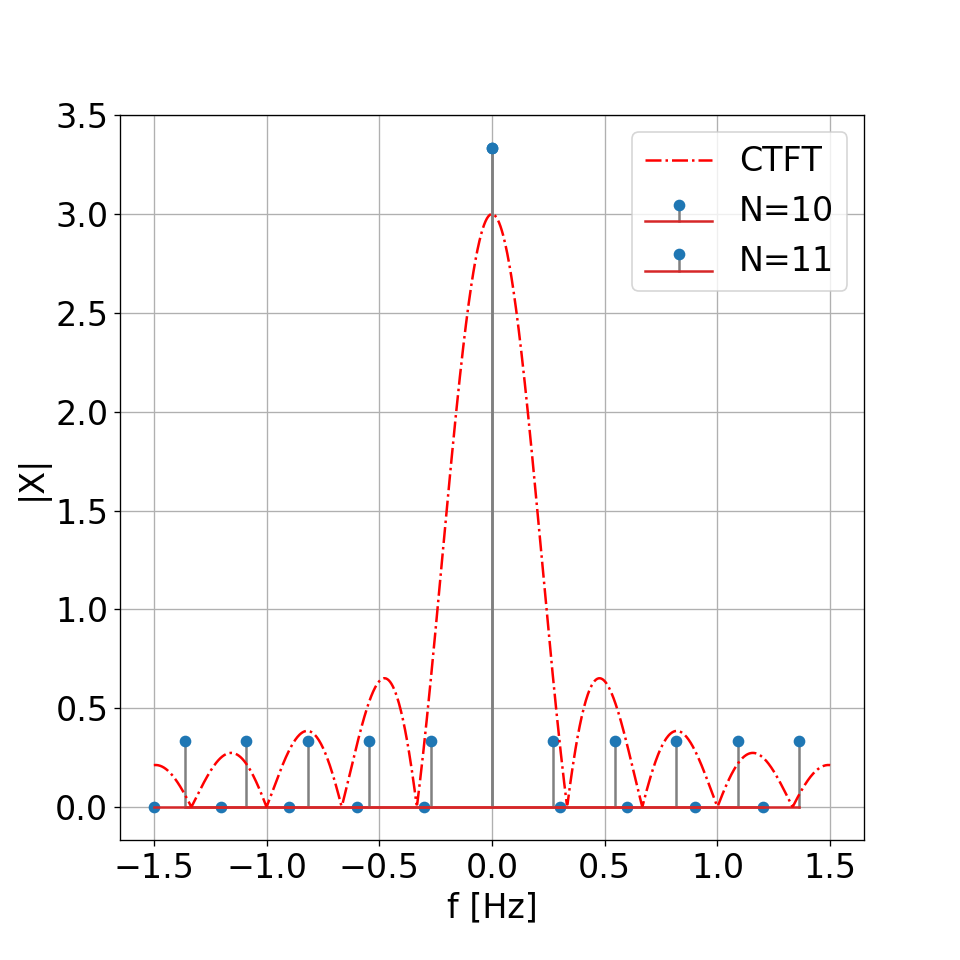
\includegraphics[width=\textwidth]{Img/punto_4_f.png}
    \caption{}
    \label{fftshift}
\end{figure}
En la figura \ref{fftshift} se aprecia que al utilizar la \textit{fftshift} las muestras de la fft no coinciden con el espectro deseado de la CTFT. Sin embargo, estas muestras son representaciones exactas de la DTFT de la señal muestreada. Esta disparidad se debe al aliasing presente en la forma de implementación de la DFT.


Para utilizar de forma correcta la \textit{fftshift} se deben cumplir las condiciones propuestas en la sección \ref{secc4c}. Esto permite obtener una visualización que se aproxime de mejor 
forma al espectro de la CTFT.


%G
 \subsection{Estimación de la CTFT a partir de la DFT}
 Para el cálculo de la CTFT utilizando la DFT se realizan los siguientes pasos:
 \begin{itemize}
     \item Obtener la señal $x[n]$ muestreando la señal $x(t)$ con una frecuencia $F_s$ que cumpla el teorema de muestreo.
     \item Implementar el algoritmo de la fft a la señal muestreada.
     \item Normalizar el resultado obtenido de la fft dividiendo por $F_s$.
     \item Filtrar un período del espectro obtenido de la DFT.
 \end{itemize}

No obstante, para obtener una aproximación exacta se deben cumplir las condiciones analizadas en la sección \ref{secc4c}.
Por último, el efecto del método zero-padding tiene como finalidad mejorar la visualización del espectro, sin alterar la información existente.


\begin{thebibliography}{0}
  \bibitem{DM}  Dimitris Manolakiv and Vinay Ingle - ``Applied Digital Signal Processing'' 5th Edition
\end{thebibliography}


\end{document}